%% Related Work
%%=========================================

\chapter{Related Work}
\label{ch:related_work}
With the relevance to natural language processing, we now present related works in the field of machine translation. This chapter presented some systems and approaches used in machine translation problems. We will also look closer at its architecture and implementation.

\section{Statistical Machine Translation}
\begin{figure}[ht]
    \centering
    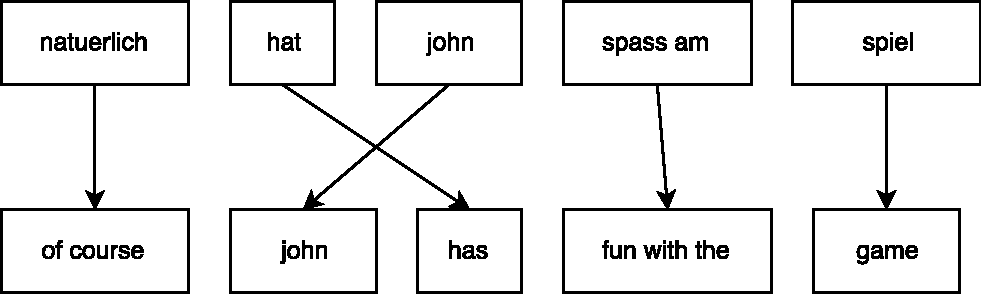
\includegraphics[width=0.7\textwidth]{fig/related_work/translation_de_en.pdf}
    \caption{Phrase-based translation of a German sentence to English. Illustration from \citep{koehn2010statistical}}
    \label{fig:translation-phrase-based}
\end{figure}

For the past two decades or so, machine translation has taken a new direction. Instead of pre-defined rule-based systems, many modern machine translation systems attack the problem of machine translation with statistical methods and ideas from information theory \citep{brown1990statistical}. Statistical machine translation was born as an idea in the 1980s in the labs of IBM Research. The idea came in the wake of success of statistical methods in speech recognition. The idea was to model the translation task as a statistical optimization problem. Some of the best performing SMT systems today are phrase-based, an approach where the input sequence is broken up into a sequence of phrases, and these phrases are mapped one-to-one to output phrases, which may be reordered \citep{koehn2010statistical}. See Figure \ref{fig:translation-phrase-based} for illustration of a phrase-based translation of a German sentence to English.

Statistical machine translation has been the dominant translation paradigm for decades \citep{wu2016google}. Variants and implementations of SMT based systems have achieved state of the art performance in machine translation \citep{watanabe07onlinelargemargin}. There now also exists SMT systems on the commercial market, a market long dominated by the well-established rule-based methods \citep{hutchins2007machine}.

%%=========================================

\section{Neural Machine Translation}
Neural machine translation is another approach to machine translation that has emerged recently. This approach aims at building a jointly-tuned single neural network which is trained to maximize translation performance. This is a different approach from traditional statistical machine translation systems, where a translation system consists of sub components that are optimized separately \citep{wolk2015neural}. The great benefit of neural machine translation systems is its ability to learn directly, in an end-to-end fashion. 

In 2016, Google published their work on Google's Neural Machine Translation system, or GNMT for short. This system \citep{wu2016google}.

%%=========================================

\section{Neural Network}
At the base of the neural machine translation systems are neural networks. The idea of models using artificial neurons, can be traced back to the 1940s. Since then, more sophisticated proposals and variants have been made from decade to decade. Artificial neural networks are an attempt at modeling the information process capabilities of nervous systems, found in the brain.

\begin{figure}[ht]
    \centering
    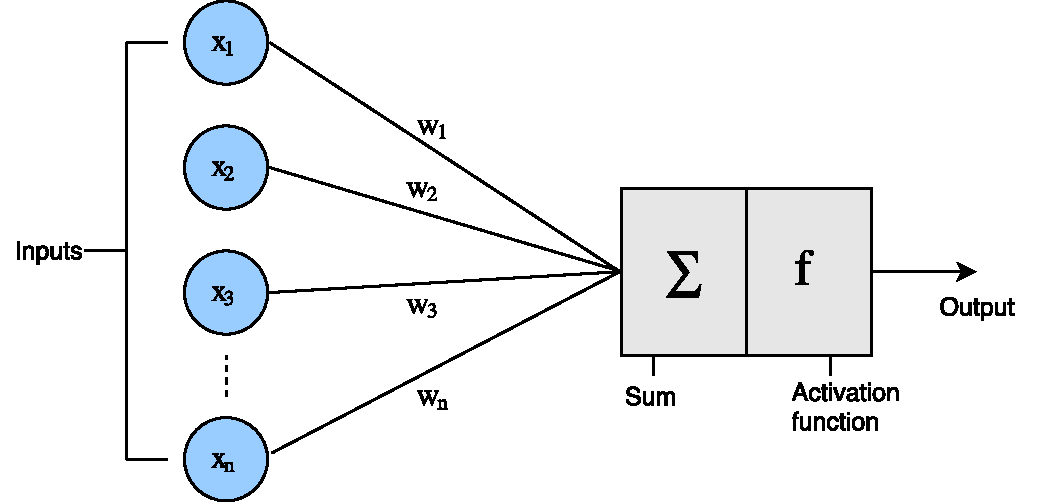
\includegraphics[width=0.7\textwidth]{fig/related_work/nn_perceptron.pdf}
    \caption{Illustration of a perceptron}
    \label{fig:nn-perceptron}
\end{figure}

\subsection{Recurrent Neural Network}
\begin{figure}[ht]
    \centering
    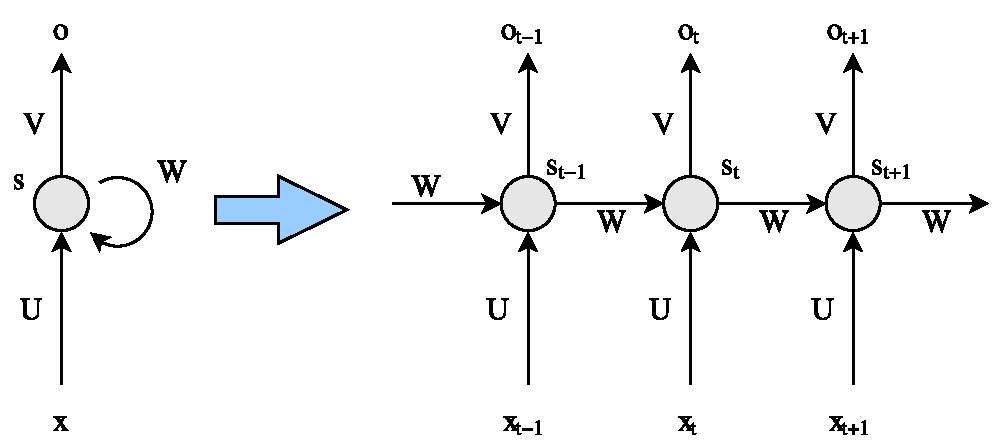
\includegraphics[width=0.7\textwidth]{fig/related_work/nn_recurrent.pdf}
    \caption{RNN unrolled}
    \label{fig:nn-rnn}
\end{figure}

\iffalse
\section{Notes}


Amazing results:
Within three years of invention, outperforming models
developed over the past 15 years, and deployed in
commercial systems
- Incredibly simple implementation:
Traditional machine translation (e.g. 6k lines of Python)
Neural machine translation (e.g. 280 lines of Python)
- Machine translation as machine learning:
Easy to apply new machine techniques directly

http://www.cs.cmu.edu/~tbergkir/11711fa16/neubig16afnlp.pdf

\subsection{Other things}
Statistical machine translation (SMT) is a machine translation paradigm where translations are generated on the basis of statistical models whose parameters are derived from the analysis of bilingual text corpora. The statistical approach contrasts with the rule-based approaches to machine translation as well as with example-based machine translation. - https://en.wikipedia.org/wiki/Statistical\_machine\_translation



\subsection{5346}
Deep Neural Networks (DNNs) are powerful models that have achieved excel- lent performance on difficult learning tasks. Although DNNs work well whenever large labeled training sets are available, they cannot be used to map sequences to sequences. (5346)

Almost better than the current state of the art. SMT syste (?) research this. 5346.

5346, reuse cite 13, 7, DNNs good results on speech recognition.

Despite their flexibility and power, DNNs can only be applied to problems whose inputs and targets can be sensibly encoded with vectors of fixed dimensionality. It is a significant limitation, since many important problems are best expressed with sequences whose lengths are not known a-priori. For example, speech recognition and machine translation are sequential problems. Likewise, ques- tion answering can also be seen as mapping a sequence of words representing the question to a sequence of words representing the answer. It is therefore clear that a domain-independent method that learns to map sequences to sequences would be useful. 5346

There have been a number of related attempts to address the general sequence to sequence learning problem with neural networks. Our approach is closely related to Kalchbrenner and Blunsom [18] who were the first to map the entire input sentence to vector, and is very similar to Cho et al. [5]. Graves [10] introduced a novel differentiable attention mechanism that allows neural networks to focus on different parts of their input, and an elegant variant of this idea was successfully applied to machine translation by Bahdanau et al. [2]. The Connectionist Sequence Classification is another popular technique for mapping sequences to sequences with neural networks, although it assumes a monotonic alignment between the inputs and the outputs [11]. 5346

Third, we found it extremely valuable to reverse the order of the words of the input sentence. So for example, instead of mapping the sentence a,b,c to the sentence $\alpha, \beta, \gamma$, the LSTM is asked to map c,b,a to $\alpha, \beta, \gamma$, where $\alpha, \beta, \gamma$ is the translation of a, b, c. This way, a is in close proximity to $\alpha$, b is fairly close to $\beta$, and so on, a fact that makes it easy for SGD to “establish communication” between the input and the output. We found this simple data transformation to greatly boost the performance of the LSTM.

%%=========================================

\section{Recurrent Neural Network}
Sequence to sequence type problems have been solve

Traditional neural networks assume and inputs and outputs are independent on each other. While this is true for some problems, for other problems there is a direct connection between earlier input and following output. Recurrent Neural Networks were designed around this relationship.

Recurrent Neural Networks, or RNNs, are a class of artificial neural networks with special characteristics. Due to how RNNs have their connections between the units, it is capable of storing an internal state for the network. This state can be used to ``remember" previous outputs and computations. This makes it possible to evaluate input on the basis of previous knowledge and apply this to the output. Recurrent in Recurrent Neural Networks, means that the calculating task is done recurrent for the input.

\red{Figure here}

Because RNNs have a concept of memory and time, it is able to use previous input and feed the knowledge from that back into its internal state. 

\subsection{Use of RNNs}
\red{TODO}

%%=========================================

\section{Variations of RNNs}
\red{TODO}

\subsection{Long Short Term Memory}
Long Short Term Memory, or LSTM for short, is a method that improves on storing information over extended time in recurrent networks. 

Recurrent does, 

\cite{hochreiter1997long}

\subsection{GRU}
\red{TODO}

%%=========================================

\section{Encoder/Decoder}
\red{TODO}

\cite{rocktaschel2015reasoning}
\fi